%! TEX program = pdflatex

\documentclass[oneside,solution]{android-assign}

\usepackage[utf8]{inputenc}
\usepackage[english,ukrainian]{babel}

\title{Підсумкова Робота}
\author{Захаров Дмитро}
\studentID{МП-31}
\instructor{Величко О.М.}
\date{\today}
\duedate{23:59 28 квітня, 2024}
\assignno{}
\semester{Весняний семестр 2024}
\mainproblem{Підсумкова робота}

% general settings for listing
\usepackage{listings}
\usepackage[many]{tcolorbox}
\definecolor{middlegray}{rgb}{0.5,0.5,0.5}
\lstset{
    xleftmargin=1.1cm,
    belowskip=2em,
    basicstyle=\fontsize{10}{15}\ttfamily,
    basewidth  = {.5em,0.4em},
    captionpos=t,
    lineskip={2pt},
    backgroundcolor=\color{white},
    framextopmargin=6pt,
    framexrightmargin=0pt,
    framexleftmargin=0.9em,    
    framexbottommargin=6pt, 
    frame=l,
%    frame=single,        
%    frame=tb, framerule=0pt,    
    framesep=6.5mm,
    fillcolor=\color{white},
    rulecolor=\color{middlegray},
    numbers=left,
    numberstyle=\normalfont\color{middlegray},
%    numberstyle=\footnotesize,    
    numbersep=10pt,
    abovecaptionskip=10pt, %space above the caption
    belowcaptionskip=10pt, %space below the caption
    extendedchars=true,
    showstringspaces=false,
    showspaces=false,
    stepnumber=1, % the step between two line-numbers. If it is 1 each line will be numbered
    tabsize=2,
    breaklines=true,
    showtabs=false,
    upquote=true,
    % German umlauts
    literate=%
    {Ö}{{\"O}}1
    {Ä}{{\"A}}1
    {Ü}{{\"U}}1
    {ß}{{\ss}}1
    {ü}{{\"u}}1
    {ä}{{\"a}}1
    {ö}{{\"o}}1
}

% define language
\lstdefinelanguage{JavaScript}{
    keywords={typeof, new, true, false, catch, then, function, return, null, catch, switch, var, if, in, while, do, else, case, break, default},
    keywordstyle=\color{editorGreen}\bfseries,
    ndkeywords={class, export, boolean, throw, implements, import, this, const},
    ndkeywordstyle=\color{vscodeblue}\bfseries,
    identifierstyle=\color{black},
    sensitive=false,
    comment=[l]{//},
    morecomment=[s]{/*}{*/},
    commentstyle=\color{editorGreen}\ttfamily,
    stringstyle=\color{darkred}\ttfamily,
    morestring=[b]',
    morestring=[b]"
}

\lstdefinelanguage{SQL}{
    keywords={select, where, from},
    keywordstyle=\color{editorGreen}\bfseries,
    ndkeywords={},
    ndkeywordstyle=\color{vscodeblue}\bfseries,
    identifierstyle=\color{black},
    sensitive=false,
    comment=[l]{--},
    morecomment=[s]{/*}{*/},
    commentstyle=\color{editorGreen}\ttfamily,
    stringstyle=\color{darkred}\ttfamily,
    morestring=[b]',
    morestring=[b]"
}


\lstdefinelanguage{HTML5}{
  language=html,
  sensitive=true,	
  alsoletter={<>=-},	
  morecomment=[s]{<!-}{-->},
  tag=[s],
  otherkeywords={
  % General
  >,
  % Standard tags
	<!DOCTYPE,
  </html, <html, <head, <title, </title, <style, </style, <link, </head, <meta, />,
	% body
	</body, <body,
	% Divs
	</div, <div, </div>, 
	% Paragraphs
	</p, <p, </p>,
	% scripts
	</script, <script,
  % More tags...
  <canvas, /canvas>, <svg, <rect, <animateTransform, </rect>, </svg>, <video, <source, <iframe, </iframe>, </video>, <image, </image>, <header, </header, <article, </article
  },
  ndkeywords={
  % General
  =,
  % HTML attributes
  charset=, src=, id=, width=, height=, style=, type=, rel=, href=,
  % SVG attributes
  fill=, attributeName=, begin=, dur=, from=, to=, poster=, controls=, x=, y=, repeatCount=, xlink:href=,
  % properties
  margin:, padding:, background-image:, border:, top:, left:, position:, width:, height:, margin-top:, margin-bottom:, font-size:, line-height:,
	% CSS3 properties
  transform:, -moz-transform:, -webkit-transform:,
  animation:, -webkit-animation:,
  transition:,  transition-duration:, transition-property:, transition-timing-function:,
  }
}

\lstdefinestyle{html} {%
  % Code design
  keywordstyle=\color{lightblack}\bfseries,
  ndkeywordstyle=\color{lightblack}\bfseries,
  identifierstyle=\color{lightblack},
  commentstyle=\color{green}\ttfamily,
  stringstyle=\color{darkred}\ttfamily,
  % Code
  language=HTML5,
%  alsolanguage=JavaScript,
  alsodigit={.:;},	
  tabsize=2,
  showtabs=false,
  showspaces=false,
  showstringspaces=false,
  extendedchars=true,
  breaklines=true,
  % German umlauts
  literate=%
  {Ö}{{\"O}}1
  {Ä}{{\"A}}1
  {Ü}{{\"U}}1
  {ß}{{\ss}}1
  {ü}{{\"u}}1
  {ä}{{\"a}}1
  {ö}{{\"o}}1
}

\lstdefinelanguage{CSS} 
{morekeywords={color,background,margin,padding,margin,padding,font,weight,display,position,top,left,right,bottom,list,style,border,size,white,space,min,width, 	transition}, 
	sensitive=false, 
	morecomment=[l]{//}, 
	morecomment=[s]{/*}{*/}, 
	morestring=[b]", 
}

\lstdefinestyle{css} {%
  language=CSS,
  keywordstyle=\color{lightblack},
}

\lstdefinestyle{js} {
  language=JavaScript
}

\lstdefinestyle{sql} {
  language=SQL,
  keywordstyle=\color{azure}  
}

\begin{document}

\maketitle

\subsection{Вступ} Цей документ дещо неформально описує процес розробки підсумкового міні-проекту, які інструменти було використано та короткий аналіз коду. Також тут ми наводимо майже повний перелік коду. Щоб погратися з самим додатком, можна перейти за наступним посиланням на \textit{GitHub} репозиторій (також там є скріншоти додатку):

\begin{center}
\url{https://github.com/ZamDimon/android-course}
\end{center}

\textbf{Умова завдання.} Побудувати графік функції
\begin{equation*}
    y(t) = \sin \omega t + \cos \omega t,
\end{equation*}

де користувач може налаштовувати параметри циклічної частоти $\omega$, а також відрізок $t \in [t_0,t_1]$, на якому малювати графік.

\subsection{Реалізація базової задачі}

Як і було запропоновано в основному курсі лекцій, ми використали пакет \texttt{androidplot}. Також, щоб було трошки легше жити, ми додали пакет \texttt{androidx.databinding:databinding-compiler}, котрий дозволяє викликати компоненти layout'а не через \texttt{findViewById}, а напряму, використовуючи \texttt{binding}. Далі опишемо основні частини додатку.

\subsubsection{Layout.} Наш layout складається з наступних 6 основних компонент:
\begin{itemize}
    \item \texttt{topAppBar} -- бар, на якому знаходиться назва додатку, а також кнопки зберегти, імпортувати та поставити дефолтні значення.
    \item \texttt{plot} -- власне наш графік, на якому ми будемо малювати синусоїду.
    \item \texttt{frequency\_slider\_label} та \texttt{frequency\_slider} -- слайдер з підписом зверху, на якому ми будемо обирати циклічну частоту.
    \item \texttt{x\_limits\_slider\_label} та \texttt{x\_limits\_slider} -- слайдер з межами по вісі $x$ (або часу).
\end{itemize}

Отже, наведемо сам layout нижче. Також, на Рисунку \ref{fig:layout} можна побачити наш Layout візуально.
\begin{figure}
    \centering
    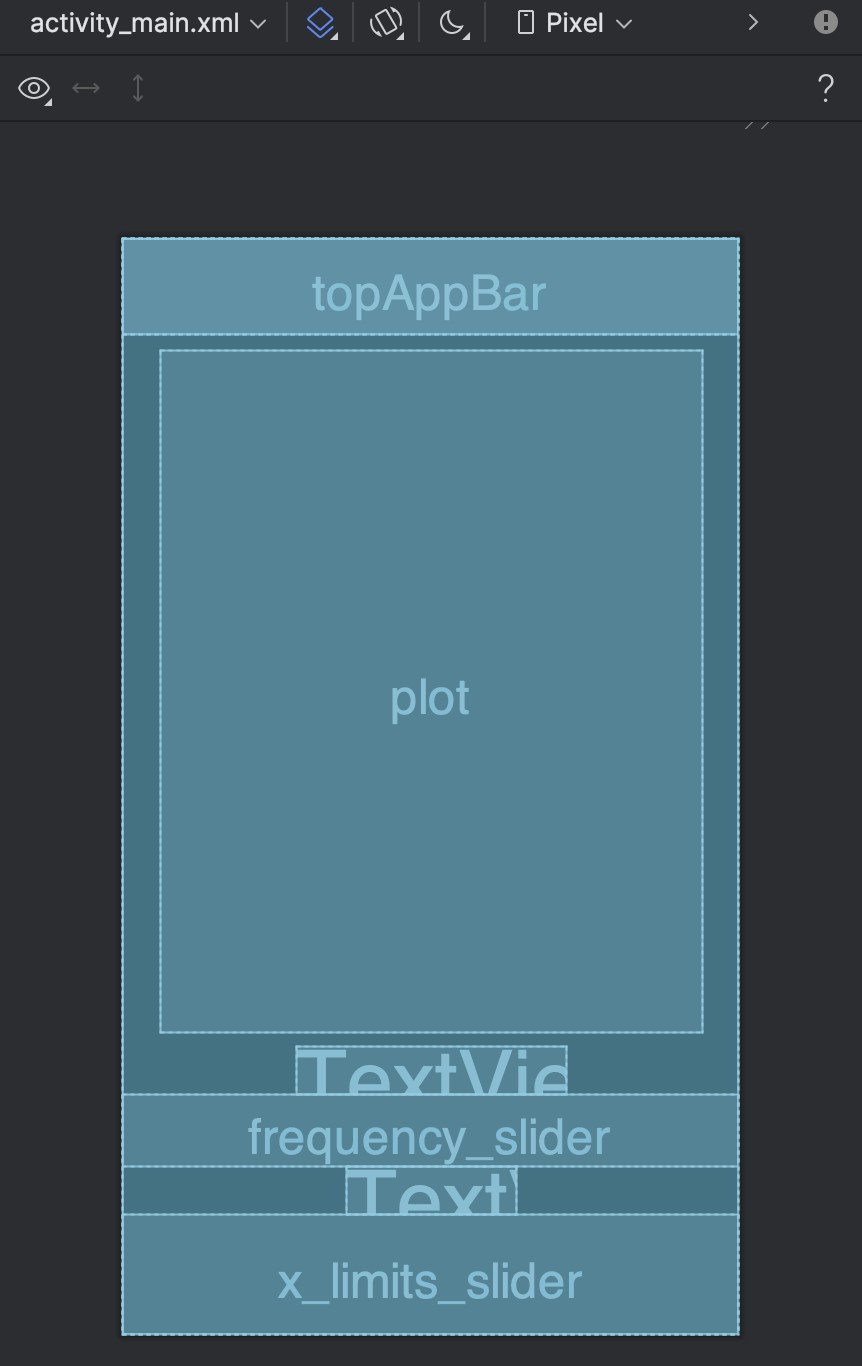
\includegraphics[width=0.8\textwidth]{screenshots/layout.png}
    \caption{Layout нашого додатку з \textit{Android Studio}.}
    \label{fig:layout}
\end{figure}

\begin{lstlisting}[language=xml]
<?xml version="1.0" encoding="utf-8"?>
<layout xmlns:android="http://schemas.android.com/apk/res/android"
    xmlns:app="http://schemas.android.com/apk/res-auto"
    xmlns:tools="http://schemas.android.com/tools">

    <data></data>

    <androidx.constraintlayout.widget.ConstraintLayout
        android:id="@+id/main"
        android:layout_width="match_parent"
        android:layout_height="match_parent"
        tools:context=".MainActivity">

        <com.google.android.material.appbar.AppBarLayout
            android:id="@+id/appBarLayout"
            android:layout_width="match_parent"
            android:layout_height="wrap_content"
            android:background="@color/material_dynamic_tertiary80"
            app:layout_constraintTop_toTopOf="parent">

            <com.google.android.material.appbar.MaterialToolbar
                android:id="@+id/topAppBar"
                android:layout_width="match_parent"
                android:layout_height="wrap_content"
                android:minHeight="?attr/actionBarSize"
                app:title="@string/main_page_title"
                app:subtitle="@string/main_page_subtitle"
                app:menu="@menu/top_app_bar" />

        </com.google.android.material.appbar.AppBarLayout>

        <com.androidplot.xy.XYPlot
            style="@style/CustomPlotStyle.Pinkish"
            android:id="@+id/plot"
            android:layout_width="0dp"
            android:layout_height="0dp"
            android:layout_marginTop="10dp"
            android:layout_marginLeft="25dp"
            android:layout_marginRight="25dp"
            android:layout_marginBottom="10dp"
            android:layout_weight="1"
            app:domainTitle="domain"
            app:layout_constraintBottom_toTopOf="@+id/frequency_slider_label"
            app:layout_constraintTop_toBottomOf="@+id/appBarLayout"
            app:layout_constraintEnd_toEndOf="parent"
            app:layout_constraintHorizontal_bias="0.5"
            app:layout_constraintStart_toStartOf="parent"
            app:lineLabelRotationBottom="-45"
            app:lineLabels="left|bottom|right"
            app:rangeTitle="range"
            app:title="Plot"
            />

        <TextView
            android:id="@+id/frequency_slider_label"
            android:layout_width="wrap_content"
            android:layout_height="wrap_content"
            app:layout_constraintTop_toBottomOf="@+id/plot"
            app:layout_constraintBottom_toTopOf="@+id/frequency_slider"
            app:layout_constraintEnd_toEndOf="parent"
            app:layout_constraintStart_toStartOf="parent"
            android:textSize="24sp"
            android:text="@string/sliders_frequency_slider_label" />

        <com.google.android.material.slider.RangeSlider
            android:id="@+id/frequency_slider"
            android:contentDescription="@string/sliders_frequency_slider_description"
            android:layout_width="match_parent"
            android:layout_height="12dp"
            android:stepSize="0.1"
            android:valueFrom="-3.0"
            android:valueTo="3.0"
            app:layout_constraintBottom_toTopOf="@+id/limits_slider_label"
            app:layout_constraintEnd_toEndOf="parent"
            app:layout_constraintStart_toStartOf="parent" />

        <TextView
            android:id="@+id/limits_slider_label"
            android:layout_width="wrap_content"
            android:layout_height="wrap_content"
            app:layout_constraintBottom_toTopOf="@+id/x_limits_slider"
            app:layout_constraintEnd_toEndOf="parent"
            app:layout_constraintStart_toStartOf="parent"
            android:textSize="24sp"
            android:text="@string/sliders_limits_slider_label" />

        <com.google.android.material.slider.RangeSlider
            android:id="@+id/x_limits_slider"
            android:contentDescription="@string/sliders_limits_slider_description"
            android:layout_width="match_parent"
            android:layout_height="12dp"
            android:stepSize="0.1"
            android:valueFrom="-5.0"
            android:valueTo="5.0"
            app:labelBehavior="withinBounds"
            app:layout_constraintBottom_toBottomOf="parent"
            app:layout_constraintEnd_toEndOf="parent"
            app:layout_constraintStart_toStartOf="parent" />

    </androidx.constraintlayout.widget.ConstraintLayout>
</layout> 
\end{lstlisting}

\subsubsection{HarmonicConfig.} Далі буде дуже зручно зберігати інформацію про графік у вигляді допоміжного класу \texttt{HarmonicConfig}. В ньому ми і покладемо наші межі та циклічну частоту. Клас виглядає наступним чином:
\begin{lstlisting}[language=java]
package com.zamdimon.graph_plotting.logic;

public class HarmonicConfig {
    /** Represents the minimal left value the plot can start drawing from. */
    public static final float MIN_LEFT_LIMIT = -5.0f;

    /** Represents the maximal right value the plot can end drawing up. */
    public static final float MAX_RIGHT_LIMIT = 5.0f;

    /** Represents the default cyclic frequency available by default */
    public static final float DEFAULT_CYCLIC_FREQUENCY = 1.0f;

    /** Represents the left x limit from which to draw the plot */
    private float leftLimit;
    /** Represents the right x limit until which to draw the plot */
    private float rightLimit;
    /** Represents the cyclic frequency of the function */
    private float cyclicFrequency;

    /**
     * Constructs the config with default values
     */
    public HarmonicConfig() {
        this.leftLimit = MIN_LEFT_LIMIT;
        this.rightLimit = MAX_RIGHT_LIMIT;
        this.cyclicFrequency = DEFAULT_CYCLIC_FREQUENCY;
    }

    /**
     * Constructor for the HarmonicPlot class with the specified fields.
     * @param leftLimit the left x limit from which to draw the plot
     * @param rightLimit the right x limit until which to draw the plot
     * @param cyclicFrequency the cyclic frequency of the function
     */
    public HarmonicConfig(float leftLimit, float rightLimit, float cyclicFrequency) {
        this.leftLimit = leftLimit;
        this.rightLimit = rightLimit;
        this.cyclicFrequency = cyclicFrequency;
    }

    /**
     * Updates the cyclic frequency of the function.
     * @param cyclicFrequency the new cyclic frequency of the function
     */
    public void updateCyclicFrequency(float cyclicFrequency) {
        this.cyclicFrequency = cyclicFrequency;
    }

    /**
     * Updates the left and right limits of the plot.
     * @param leftLimit the new left x limit from which to draw the plot
     * @param rightLimit the new right x limit until which to draw the plot
     */
    public void updateLimits(float leftLimit, float rightLimit) {
        assert rightLimit > leftLimit : "Right limit must be greater than the left one";

        this.leftLimit = leftLimit;
        this.rightLimit = rightLimit;
    }

    /**
     * @return Left x limit from which to draw the plot
     */
    public float getLeftLimit() {
        return leftLimit;
    }

    /**
     * @return Right x limit until which to draw the plot
     */
    public float getRightLimit() {
        return rightLimit;
    }

    /**
     * @return Length of the plot along the Ox axis
     */
    public float getLimitLength() {
        return rightLimit - leftLimit;
    }

    /**
     * @return the cyclic frequency of the function
     */
    public float getCyclicFrequency() {
        return cyclicFrequency;
    }
}
\end{lstlisting}

Насправді доволі простий клас, в котрому є аксесори до параметрів, а також методи для їх оновлення, ініціалізації, а також підтримка публічних константних значень, що відповідають дефолтним значенням відповідних полів.

\subsubsection{HarmonicPlot.} Тут найцікавіше, це власне клас, в якому ми будемо будувати і малювати графік. Виглядає він наступним чином:
\begin{lstlisting}[language=java]
package com.zamdimon.graph_plotting.logic;

import android.graphics.Color;
... (other imports)

/**
 * Class responsible for internal logic needed to display a plot.
 */
public class HarmonicPlot {
    /** Function which is being plotted. By default, as the problem suggests,
     * we draw a function sin(omega*x) + cos(omega*x) */
    private Function<Float, Float> function = x -> (float) (Math.sin(x) + Math.cos(x));

    /** Configuration file of our plot. Contains the core data such as frequency or x limits. */
    private final HarmonicConfig config;

    /**
     * Sets the function to be plotted.
     * @param function the new function to be plotted
     */
    public void setFunction(Function<Float, Float> function) {
        this.function = function;
    }

    /**
     * Constructs the HarmonicPlot with default parameters
     */
    public HarmonicPlot() {
        this.config = new HarmonicConfig();
    }

    /**
     * Contructs the HarmonicPlot with specified config
     * @param config Config to initialize the plot with
     */
    public HarmonicPlot(@NonNull HarmonicConfig config) {
        this.config = config;
    }

    /**
     * Updates the limit of the internal config
     * @param leftLimit coordinate from which to start drawing the plot
     * @param rightLimit coordinate until which to draw the plot
     */
    public void updateLimits(float leftLimit, float rightLimit) {
        config.updateLimits(leftLimit, rightLimit);
    }

    /**
     * Updates the cyclic frequency of the internal config
     * @param frequency the new cyclic frequency of the function
     */
    public void updateCyclicFrequency(float frequency) {
        config.updateCyclicFrequency(frequency);
    }

    /**
     * Estimates the number of points needed to draw the plot.
     * @return the estimated number of points needed to draw the plot
     */
    private int estimatePointsNumber() {
        float period = 2 * (float) Math.PI / config.getCyclicFrequency();
        // We want approximately 8 points per period. Meaning, the total
        // number of points is the total number of periods in the specified
        // interval multiplied by 8.
        float periods = config.getLimitLength() / period;
        // We want at least 10 points, otherwise adapt according to the number
        // of periods.
        final int POINTS_PER_PERIOD = 35;
        final int MIN_POINTS = 35;
        return Math.max((int) (periods * POINTS_PER_PERIOD), MIN_POINTS);
    }

    /**
     * Forms the plot points for the plot.
     * @return the XYSeries representing the plot points
     */
    private @NonNull XYSeries formPlotPoints() {
        // Initializing empty lists
        List<Number> xNumbers = new ArrayList<>();
        List<Number> yNumbers = new ArrayList<>();

        int pointsNumber = this.estimatePointsNumber();
        for (int i = 0; i < pointsNumber; ++i) {
            float x = config.getLeftLimit() + config.getLimitLength() * i / pointsNumber;
            float y = function.apply(x * config.getCyclicFrequency());

            xNumbers.add(x);
            yNumbers.add(y);
        }

        final String PLOT_TITLE = "harmonic_plot";
        return new SimpleXYSeries(xNumbers, yNumbers, PLOT_TITLE);
    }

    /**
     * Draws the plot on the given XYPlot.
     * @param plot the XYPlot to draw the plot on
     */
    public void drawPlot(@NonNull XYPlot plot) {
        XYSeries series = formPlotPoints();

        final int LINE_COLOR = Color.BLUE;
        final int POINT_COLOR = Color.GREEN;
        LineAndPointFormatter pointFormatter = new LineAndPointFormatter(LINE_COLOR, POINT_COLOR, null, null);

        // Adding interpolation to make curve a little bit smoother
        final int POINTS_PER_SEGMENT = 20;
        pointFormatter.setInterpolationParams(new CatmullRomInterpolator.Params(POINTS_PER_SEGMENT, CatmullRomInterpolator.Type.Centripetal));

        // Change the line width
        final int STROKE_WIDTH = 10;
        Paint paint = pointFormatter.getLinePaint();
        paint.setStrokeWidth(STROKE_WIDTH);
        pointFormatter.setLinePaint(paint);

        // Clearing and redrawing the plot
        plot.clear();
        plot.addSeries(series, pointFormatter);
        plot.redraw();
    }
}
\end{lstlisting}

Тут варто звернути увагу на наступні речі:
\begin{itemize}
    \item Найголовніша проблема була зробити так, щоб точок на графіку було небагато (бо велику кількість обробляти дуже важко), але при цьому графік виглядав максимально гладко. Для цього був застосований вбудований в пакет інтерполятор \texttt{CatmullRomInterpolator}, а також дещо саморобний метод адаптивного підбору оптимальної кількості точок. Його ідея полягає в тому, що чим більше періодів синусоїди намальовано, тим більше точок треба наносити і навпаки. Тому, якщо в середньому потрібно 35 точок на період (емпирічно підібране значення), то приблизна загальна кількість точок задається як $\frac{t_1-t_0}{T} \times 35$.
    \item Параметри, по яким ми будуємо точки, беремо з \texttt{HarmonicConfig}.
    \item Також ми зробили сам графік трошки жирнішим за допомогою методу $\texttt{.setStrokeWidth}$.
\end{itemize}

\subsubsection{MainActivity.} Оскільки нововедення дуже суттєво змінять логіку, сам код \texttt{MainActivity} ми наведемо пізніше після того, як опишемо нові функції.

Отже, ми маємо весь базовий функціонал! Тепер давайте пограємось і додамо щось цікавеньке.

\subsection{Нові функції.}

\subsubsection{Shared Preferences.} По-перше, було б цікаво, якщо б параметри частоти та меж зберігалися при виході з додатку. Саме тому ми додали wrapper навколо \texttt{HarmonicConfig}, котрий дозволяє зберігати преференції і підвантажувати при запуску додатку. 

Оскільки shared preferences це, по суті, звичайна key-value табличка, то зручно захардкодити ключі у вигляді імпровізованого \texttt{enum} типу:

\begin{lstlisting}[language=java]
package com.zamdimon.graph_plotting.storage;

/**
 * Represents the fields of the harmonic configuration
 * in a "sort of" enum-like type.
 */
public final class HarmonicConfigFields {
    /** Represents the left limit of the plot */
    public static final String LEFT_LIMIT = "leftLimit";
    /** Represents the right limit of the plot */
    public static final String RIGHT_LIMIT = "rightLimit";
    /** Represents the cyclic frequency of the function */
    public static final String CYCLIC_FREQUENCY = "cyclicFrequency";
}
\end{lstlisting}

А далі власне наш wrapper:
\begin{lstlisting}[language=java]
package com.zamdimon.graph_plotting.storage;

import com.zamdimon.graph_plotting.logic.HarmonicConfig;
import android.content.Context;
import android.content.SharedPreferences;

import androidx.annotation.NonNull;

/**
 * Class responsible for managing the preferences of the HarmonicConfig object.
 * Basically, it is a wrapper for HarmonicConfig which allows to save and load the configuration
 * from the SharedPreferences.
 */
public class HarmonicConfigPreferences {
    /** Name of the preferences file */
    public static final String PREFERENCES_NAME = "harmonic_config";

    /** Configuration file which is synced with the current shared preferences */
    private HarmonicConfig config;

    /**
     * Constructs the preferences wrapper. It loads the configuration from the shared preferences.
     * If the preferences are not set, it uses the default values. Updates the inner HarmonicConfig.
     * @param context the context of the application
     */
    public HarmonicConfigPreferences(@NonNull Context context) {
        SharedPreferences preferences = context.getSharedPreferences(PREFERENCES_NAME, Context.MODE_PRIVATE);
        float leftLimit = preferences.getFloat(HarmonicConfigFields.LEFT_LIMIT, HarmonicConfig.MIN_LEFT_LIMIT);
        float rightLimit = preferences.getFloat(HarmonicConfigFields.RIGHT_LIMIT, HarmonicConfig.MAX_RIGHT_LIMIT);
        float frequency = preferences.getFloat(HarmonicConfigFields.CYCLIC_FREQUENCY, HarmonicConfig.DEFAULT_CYCLIC_FREQUENCY);

        this.config = new HarmonicConfig(leftLimit, rightLimit, frequency);
    }

    /**
     * Saves the frequency to the shared preferences and updates the inner configuration.
     * @param context the context of the application
     * @param frequency the new frequency to be saved
     */
    public void saveFrequency(@NonNull Context context, float frequency) {
        SharedPreferences preferences = context.getSharedPreferences(PREFERENCES_NAME, Context.MODE_PRIVATE);
        SharedPreferences.Editor editor = preferences.edit();

        editor.putFloat(HarmonicConfigFields.CYCLIC_FREQUENCY, frequency);
        editor.apply();

        this.config.updateCyclicFrequency(frequency);
    }

    /**
     * Saves the limits to the shared preferences and updates the inner configuration.
     * @param context the context of the application
     * @param leftLimit the new left limit to be saved
     * @param rightLimit the new right limit to be saved
     */
    public void saveLimits(@NonNull Context context, float leftLimit, float rightLimit) {
        SharedPreferences preferences = context.getSharedPreferences(PREFERENCES_NAME, Context.MODE_PRIVATE);
        SharedPreferences.Editor editor = preferences.edit();

        editor.putFloat(HarmonicConfigFields.LEFT_LIMIT, leftLimit);
        editor.putFloat(HarmonicConfigFields.RIGHT_LIMIT, rightLimit);
        editor.apply();

        this.config.updateLimits(leftLimit, rightLimit);
    }

    /**
     * Saves the configuration to the shared preferences.
     * @param context the context of the application
     * @param config the configuration to be saved
     */
    public void saveConfig(@NonNull Context context, HarmonicConfig config) {
        SharedPreferences preferences = context.getSharedPreferences(PREFERENCES_NAME, Context.MODE_PRIVATE);
        SharedPreferences.Editor editor = preferences.edit();

        editor.putFloat(HarmonicConfigFields.LEFT_LIMIT, config.getLeftLimit());
        editor.putFloat(HarmonicConfigFields.RIGHT_LIMIT, config.getRightLimit());
        editor.putFloat(HarmonicConfigFields.CYCLIC_FREQUENCY, config.getCyclicFrequency());
        editor.apply();

        this.config = config;
    }

    /**
     * @return the current configuration
     */
    public HarmonicConfig getConfig() {
        return config;
    }
}
\end{lstlisting}

По суті, \texttt{HarmonicConfigPreferences} це і є \texttt{HarmonicConfig} з двома ключовими відмінностями:
\begin{itemize}
    \item В конструкторі підвантажуються значення з \texttt{SharedPreferences} або, якщо їх немає, то беруться дефолтні.
    \item Є методи на оновлення параметрів, котрі одночасно роблять запит на оновлення/створення в \texttt{SharedPreferences} і синхронізують внутрішній \texttt{this.config} зі значенням в \texttt{SharedPreferences}. Це потрібно, щоб при кожному отриманні \texttt{SharedPreferences} не потрібно було робити запитів, а просто взяти внутрішній instance класу \texttt{HarmonicConfig} (по суті кешування).
\end{itemize}

\subsubsection{Зберігання преференцій.} А було б ще цікавіше, якщо б параметри не просто зберігались локально, а їх можна було кудись викачати і потім заімпортити. Або, переслати другу файл з преференціями, а друг міг би відкрити цей файл. Тому ми вирішили розробити дві функції:
\begin{itemize}
    \item Функцію формування \texttt{json} файлу з усіма параметрами \texttt{HarmonicConfig}.
    \item Функцію читання \texttt{json} файлу, котрий може спарсити данні у \texttt{HarmonicConfig}.
\end{itemize}

Ці функції ми вирішили помістити на тулбар зверху у вигляді кнопок з іконками. Для цього ми додали наступне меню (тут є ще кнопка сбросу налаштунків, але вона не дуже цікава):
\begin{lstlisting}[language=xml]
<?xml version="1.0" encoding="utf-8"?>
<menu xmlns:android="http://schemas.android.com/apk/res/android"
    xmlns:app="http://schemas.android.com/apk/res-auto">
    <item
        android:id="@+id/reset"
        android:title="@string/toolbar_reset"
        android:icon="@drawable/reset"
        app:showAsAction="ifRoom"
        />
    <item
        android:id="@+id/save"
        android:title="@string/toolbar_save"
        android:icon="@drawable/save"
        app:showAsAction="ifRoom"
        />

    <item
        android:id="@+id/upload"
        android:icon="@drawable/upload"
        android:title="@string/toolbar_upload"
        app:showAsAction="always"
        />
</menu>
\end{lstlisting}

Іконки ми взяли з сайту \url{https://fonts.google.com/icons}. 

Тепер, для зберігання ми створили наступний клас, котрий зчитує усі kv значення з \texttt{SharedPreferences} та формує з них \texttt{.json} файл:
\begin{lstlisting}[language=java]
package com.zamdimon.graph_plotting.utils;

import android.content.Context;
import android.content.SharedPreferences;
import android.net.Uri;
import android.util.Log;

import org.json.JSONException;
import org.json.JSONObject;

import java.io.File;
import java.io.FileWriter;
import java.io.IOException;
import java.io.OutputStream;
import java.io.OutputStreamWriter;
import java.util.Map;

/**
 * Utility class for handling SharedPreferences
 */
public class SharedPreferencesUtil {
    /**
     * Converts SharedPreferences to JSON Object
     * @param context the context of the application
     * @param prefsName the name of the SharedPreferences file
     * @return JSON Object containing the SharedPreferences
     */
    public static JSONObject getSharedPreferencesAsJson(Context context, String prefsName) {
        // Retrieve SharedPreferences
        SharedPreferences sharedPreferences = context.getSharedPreferences(prefsName, Context.MODE_PRIVATE);
        Map<String, ?> allEntries = sharedPreferences.getAll();

        // Convert to JSON Object
        JSONObject jsonObject = new JSONObject();
        for (Map.Entry<String, ?> entry : allEntries.entrySet()) {
            try {
                jsonObject.put(entry.getKey(), entry.getValue());
            } catch (JSONException e) {
                Log.e("SharedPreferencesUtil", "Error putting key-value into json object", e);
            }
        }
        return jsonObject;
    }

    /**
     * Saves JSON Object to file
     * @param context the context of the application
     * @param uri the URI of the file to save
     * @param jsonObject the JSON Object to save
     */
    public static void saveJsonToFile(Context context, Uri uri, JSONObject jsonObject) {
        try {
            OutputStream outputStream = context.getContentResolver().openOutputStream(uri);
            if (outputStream != null) {
                OutputStreamWriter outputStreamWriter = new OutputStreamWriter(outputStream);
                outputStreamWriter.write(jsonObject.toString());
                outputStreamWriter.close();
                outputStream.close();
            }
        } catch (IOException e) {
            Log.e("SharedPreferencesUtil", "Error saving JSON to file", e);
        }
    }
}
\end{lstlisting}

І далі створили наступний клас, котрий ми потім вставимо в \texttt{MainActivity}. Він містить callback та intent, що потрібні для запуску меню юзера з вибором де зберігти файл, а також хендлінгу його вибору з нашої сторони.
\begin{lstlisting}[language=java]
package com.zamdimon.graph_plotting.storage;

import android.app.Activity;
import android.content.Context;
import android.content.Intent;
import android.net.Uri;
import android.widget.Toast;

import androidx.activity.result.ActivityResult;

import com.zamdimon.graph_plotting.utils.SharedPreferencesUtil;

import org.json.JSONObject;

/**
 * Helper class for managing the saving of HarmonicConfig
 */
public class HarmonicConfigSave {
    /**
     * Handles the result of the save activity
     * @param context the context of the application
     * @param result the result of the activity
     */
    public static void onSaveActivityResult(Context context, ActivityResult result) {
        if (result.getResultCode() != Activity.RESULT_OK) {
            return;
        }

        Intent data = result.getData();
        if (data == null) {
            return;
        }
        Uri createFileUri = data.getData();
        if (createFileUri == null) {
            return;
        }
        JSONObject jsonObject = SharedPreferencesUtil.getSharedPreferencesAsJson(context, HarmonicConfigPreferences.PREFERENCES_NAME);
        SharedPreferencesUtil.saveJsonToFile(context, createFileUri, jsonObject);

        // Displaying a toast
        CharSequence text = "File saved successfully!";
        int duration = Toast.LENGTH_LONG;

        Toast toast = Toast.makeText(context, text, duration);
        toast.show();
    }

    /**
     * Creates an intent for saving the .json file with preferences
     * @return the intent for saving the .json file
     */
    public static Intent formSaveIntent() {
        Intent intent = new Intent(Intent.ACTION_CREATE_DOCUMENT);
        intent.addCategory(Intent.CATEGORY_OPENABLE);
        final String MIME_TYPE = "application/json";
        intent.setType(MIME_TYPE);
        final String EXTRA_FILE_NAME = "shared_prefs.json";
        intent.putExtra(Intent.EXTRA_TITLE, EXTRA_FILE_NAME);

        return intent;
    }
}
\end{lstlisting}

Тут цікаво наступне: для того, щоб створити вікно з вибором, де зберігати файл, потрібно створити \texttt{Intent}. Далі ми його запустимо через \texttt{ResultLauncher} разом з callback у \texttt{MainActivity}.

\subsubsection{Зчитування преференцій з файлу.} Створимо клас, майже аналогічний вище наведеному. Тут багато роботи з файлової системою, що дуже нудно, тому не будемо сильно зосереджувати увагу. Єдине, тут ми використовували пакет \texttt{Gson} для десериалізації сирих данних у класові поля -- доволі зручна річ.

\begin{lstlisting}[language=java]
package com.zamdimon.graph_plotting.storage;

import android.app.Activity;
import android.content.ContentResolver;
import android.content.Context;
import android.content.Intent;
import android.net.Uri;

import androidx.activity.result.ActivityResult;
import androidx.fragment.app.FragmentManager;

import com.google.gson.Gson;
import com.zamdimon.graph_plotting.dialogs.HarmonicConfigConfirmDialog;
import com.zamdimon.graph_plotting.dialogs.HarmonicConfigErrorDialog;
import com.zamdimon.graph_plotting.logic.HarmonicConfig;

import java.io.BufferedReader;
import java.io.InputStream;
import java.io.InputStreamReader;
import java.util.function.Consumer;

/**
 * Helper class for managing the upload of HarmonicConfig
 */
public class HarmonicConfigUpload {
    /**
     * Handles the result of the upload activity
     * @param context the context of the application
     * @param result the result of the activity
     * @param fragmentManager the fragment manager
     * @param acceptCallback the callback being called when the user accepts the upload
     */
    public static void onUploadActivityResult(Context context, ActivityResult result, FragmentManager fragmentManager, Consumer<HarmonicConfig> acceptCallback) {
        if (result.getResultCode() != Activity.RESULT_OK) {
            return;
        }

        Intent data = result.getData();
        if (data == null) {
            return;
        }
        Uri chooseFileUri = data.getData();
        if (chooseFileUri == null) {
            return;
        }
        HarmonicConfig config = getFileContent(chooseFileUri, context.getContentResolver());
        if (config == null) {
            // Displaying an error
            HarmonicConfigErrorDialog errorDialog = new HarmonicConfigErrorDialog();
            final String UPLOAD_ERROR_DIALOG_TAG = "error_dialog";
            errorDialog.show(fragmentManager, UPLOAD_ERROR_DIALOG_TAG);
            return;
        }

        // Displaying a success button
        HarmonicConfigConfirmDialog dialog = new HarmonicConfigConfirmDialog(config, () -> acceptCallback.accept(config), () -> {});
        final String UPLOAD_DIALOG_TAG = "upload_dialog";
        dialog.show(fragmentManager, UPLOAD_DIALOG_TAG);
    }

    /**
     * Retrieves the content of the file in the form of HarmonicConfig
     * @param contentUri the URI of the content
     * @param contentResolver the content resolver
     * @return the HarmonicConfig object
     */
    public static HarmonicConfig getFileContent(Uri contentUri, ContentResolver contentResolver) {
        try {
            InputStream inputStream = contentResolver.openInputStream(contentUri);
            BufferedReader reader = new BufferedReader(new InputStreamReader(inputStream));
            StringBuilder content = new StringBuilder();
            String line;

            while((line = reader.readLine()) != null) {
                content.append(line);
            }

            reader.close();

            Gson gson = new Gson();
            return gson.fromJson(content.toString(), HarmonicConfig.class);
        } catch(Exception e) {
            return null;
        }
    }

    /**
     * Forms the upload intent
     * @return the upload intent
     */
    public static Intent formUploadIntent() {
        Intent chooseFile;
        Intent intent;
        chooseFile = new Intent(Intent.ACTION_GET_CONTENT);
        chooseFile.addCategory(Intent.CATEGORY_OPENABLE);
        final String MIME_TYPE = "application/json";
        chooseFile.setType(MIME_TYPE);

        final String CHOOSER_TITLE = "Choose a file";
        intent = Intent.createChooser(chooseFile, CHOOSER_TITLE);
        return intent;
    }
}
\end{lstlisting}

Проте, дещо цікаве таки є! Ми додали два діалога: \texttt{HarmonicConfigConfirmDialog} та \texttt{HarmonicConfigErrorDialog}, котрі потрібні для інформування юзера про статус обробки обраного документа. Якщо виникла помилка, то викликається діалог, що реалізований наступним чином:
\begin{lstlisting}[language=java]
package com.zamdimon.graph_plotting.dialogs;

import android.app.Dialog;
import android.content.Context;
import android.os.Bundle;

import androidx.annotation.NonNull;
import androidx.fragment.app.DialogFragment;
import androidx.fragment.app.FragmentActivity;

import com.google.android.material.dialog.MaterialAlertDialogBuilder;
import com.zamdimon.graph_plotting.R;

/**
 * Dialog that is displayed when the configuration upload fails.
 */
public class HarmonicConfigErrorDialog extends DialogFragment {
    /**
     * Creates the dialog.
     * @param savedInstanceState the saved instance state
     * @return the dialog
     */
    @NonNull
    @Override
    public Dialog onCreateDialog(Bundle savedInstanceState) {
        super.onCreateDialog(savedInstanceState);

        FragmentActivity activity = getActivity();
        assert activity != null : "Activity must not be null";

        Context context = getContext();
        assert context != null : "Context must not be null";

        MaterialAlertDialogBuilder builder = new MaterialAlertDialogBuilder(activity);
        builder.setTitle(R.string.config_upload_error_title)
                .setMessage(R.string.config_upload_error_message);

        return builder.create();
    }
}
\end{lstlisting}

Якщо ж все нормально, то в діалогу з'являються кнопки:
\begin{lstlisting}[language=java]
package com.zamdimon.graph_plotting.dialogs;

import android.app.Dialog;
import android.content.Context;
import android.os.Bundle;
import android.widget.Toast;

import androidx.annotation.NonNull;
import androidx.fragment.app.DialogFragment;
import androidx.fragment.app.FragmentActivity;

import com.google.android.material.dialog.MaterialAlertDialogBuilder;
import com.zamdimon.graph_plotting.R;
import com.zamdimon.graph_plotting.logic.HarmonicConfig;

/**
 * Dialog that is displayed when the configuration upload is successful.
 */
public class HarmonicConfigConfirmDialog extends DialogFragment {
    private final HarmonicConfig config;

    private final Runnable acceptCallback;

    private final Runnable cancelCallback;

    /**
     * Creates the dialog.
     * @param config the configuration to be displayed
     * @param acceptCallback the callback being called when the user accepts the upload
     * @param cancelCallback the callback being called when the user cancels the upload
     */
    public HarmonicConfigConfirmDialog(@NonNull HarmonicConfig config, Runnable acceptCallback, Runnable cancelCallback) {
        this.config = config;
        this.acceptCallback = acceptCallback;
        this.cancelCallback = cancelCallback;
    }

    /**
     * Forms the message of the dialog.
     * @return the message
     */
    private String formMessage() {
        return "Left limit: " + config.getLeftLimit() + "\n" +
                "Right limit: " + config.getRightLimit() + "\n" +
                "Cyclic frequency: " + config.getCyclicFrequency();
    }

    /**
     * Creates the dialog.
     * @param savedInstanceState the saved instance state
     * @return the dialog
     */
    @NonNull
    @Override
    public Dialog onCreateDialog(Bundle savedInstanceState) {
        super.onCreateDialog(savedInstanceState);

        FragmentActivity activity = getActivity();
        assert activity != null : "Activity must not be null";

        Context context = getContext();
        assert context != null : "Context must not be null";

        MaterialAlertDialogBuilder builder = new MaterialAlertDialogBuilder(activity);
        builder.setTitle(R.string.config_upload_title)
                .setMessage(formMessage())
                .setPositiveButton(R.string.config_upload_confirm, (dialog, id) -> {
                    acceptCallback.run();

                    // Displaying a toast
                    CharSequence text = "Upload successful!";
                    int duration = Toast.LENGTH_LONG;

                    Toast toast = Toast.makeText(context, text, duration);
                    toast.show();
                })
                .setNegativeButton(R.string.config_upload_cancel, (dialog, id) -> cancelCallback.run());

        return builder.create();
    }
}
\end{lstlisting}

Також, ми використали \texttt{Toast}, щоб показати юзеру повідомлення, що все пройшло успішно. Нарешті, ітоговий \textbf{MainActivity} виглядає наступним чином:
\begin{lstlisting}[language=java]
package com.zamdimon.graph_plotting;
import android.content.Context;
import android.content.Intent;
import android.content.SharedPreferences;
import android.os.Bundle;
import android.widget.Toast;

import androidx.activity.result.ActivityResultLauncher;
import androidx.activity.result.contract.ActivityResultContracts;
import androidx.appcompat.app.AppCompatActivity;
import androidx.databinding.DataBindingUtil;
import com.zamdimon.graph_plotting.databinding.ActivityMainBinding;
import com.zamdimon.graph_plotting.logic.HarmonicConfig;
import com.zamdimon.graph_plotting.logic.HarmonicPlot;
import com.zamdimon.graph_plotting.storage.HarmonicConfigPreferences;
import com.zamdimon.graph_plotting.storage.HarmonicConfigSave;
import com.zamdimon.graph_plotting.storage.HarmonicConfigUpload;

/**
 * Main activity of the application. It is responsible for managing the UI and the logic of the application.
 */
public class MainActivity extends AppCompatActivity {
    /** Represents the binding of the activity which makes
     * it easier to manage elements of the activity */
    private ActivityMainBinding binding;

    /** Represents the preferences of the harmonic plot - basically, the settings */
    private HarmonicConfigPreferences plotPreferences;

    /**
     * Called when the activity is starting.
     * @param savedInstanceState If the activity is being re-initialized after
     *     previously being shut down then this Bundle contains the data it most
     *     recently supplied in {@link #onSaveInstanceState}.  <b><i>Note: Otherwise it is null.</i></b>
     */
    @Override
    protected void onCreate(Bundle savedInstanceState) {
        super.onCreate(savedInstanceState);
        binding = DataBindingUtil.setContentView(this, R.layout.activity_main);

        Context context = getApplicationContext();

        // Setting the harmonic plot
        plotPreferences = new HarmonicConfigPreferences(context);
        displayPlot();

        // Setting the top bar
        initializeTopBarMenu();

        // Setting sliders
        initializeFrequencySlider();
        initializeLimitsSlider();

        // Setting updating plot when shared preferences get modified
        subscribeOnSharedPreferenceChanges();
    }

    /**
     * Initializes the limits slider and subscribes to its changes.
     */
    private void initializeLimitsSlider() {
        // Setting limits from preferences
        float initialLeftLimit = plotPreferences.getConfig().getLeftLimit();
        float initialRightLimit = plotPreferences.getConfig().getRightLimit();
        binding.xLimitsSlider.setValues(initialLeftLimit, initialRightLimit);

        // Setting the minimum separation between the limits to avoid cases
        // when left limit is exactly the right limit
        final float MIN_SEPARATION = 0.3f;
        binding.xLimitsSlider.setMinSeparationValue(MIN_SEPARATION);

        // Subscribing to updating the limits
        binding.xLimitsSlider.addOnChangeListener((slider, value, fromUser) -> {
            Context context = getApplicationContext();
            float leftLimit = binding.xLimitsSlider.getValues().get(0);
            float rightLimit = binding.xLimitsSlider.getValues().get(1);
            plotPreferences.saveLimits(context, leftLimit, rightLimit);
        });
    }

    /**
     * Refreshes the sliders with the values from the preferences.
     */
    public void refreshSliders() {
        float initialLeftLimit = plotPreferences.getConfig().getLeftLimit();
        float initialRightLimit = plotPreferences.getConfig().getRightLimit();
        binding.xLimitsSlider.setValues(initialLeftLimit, initialRightLimit);

        float initialCyclicFrequency = plotPreferences.getConfig().getCyclicFrequency();
        binding.frequencySlider.setValues(initialCyclicFrequency);
    }

    /**
     * Initializes the frequency slider and subscribes to its changes.
     */
    private void initializeFrequencySlider() {
        // Setting frequency from preferences
        float initialCyclicFrequency = plotPreferences.getConfig().getCyclicFrequency();
        binding.frequencySlider.setValues(initialCyclicFrequency);

        // Subscribing to updating the frequency
        binding.frequencySlider.addOnChangeListener((rangeSlider, frequency, b) -> {
            Context context = getApplicationContext();
            plotPreferences.saveFrequency(context, frequency);
        });
    }

    /**
     * Subscribes to shared preferences changes and updates the plot when they change.
     */
    private void subscribeOnSharedPreferenceChanges() {
        SharedPreferences preferences = getSharedPreferences(HarmonicConfigPreferences.PREFERENCES_NAME, Context.MODE_PRIVATE);
        preferences.registerOnSharedPreferenceChangeListener((sharedPreferences, key) -> displayPlot());
    }

    /**
     * Displays the plot on the screen.
     */
    private void displayPlot() {
        HarmonicConfig config = plotPreferences.getConfig();
        HarmonicPlot plot = new HarmonicPlot(config);
        plot.drawPlot(binding.plot);
    }

    /**
     * Registers the activity result launcher for saving the file.
     */
    private final ActivityResultLauncher<Intent> saveFileResultLauncher = registerForActivityResult(
            new ActivityResultContracts.StartActivityForResult(),
            result -> HarmonicConfigSave.onSaveActivityResult(getApplicationContext(), result)
    );

    /**
     * Registers the activity result launcher for uploading the file.
     */
    private final ActivityResultLauncher<Intent> uploadFileResultLauncher = registerForActivityResult(
            new ActivityResultContracts.StartActivityForResult(),
            result -> HarmonicConfigUpload.onUploadActivityResult(getApplicationContext(), result, getSupportFragmentManager(), (HarmonicConfig config) -> {
                // NOTE: it is quite painful to pass all the necessary parameters inside
                // the HarmonicConfigUpload class, so we just pass the Consumer to the method
                plotPreferences.saveConfig(getApplicationContext(), config);
                displayPlot();
                refreshSliders();
            }));

    /**
     * Initializes the top bar menu.
     */
    private void initializeTopBarMenu() {
        binding.topAppBar.setOnMenuItemClickListener(item -> {
            if (item.getItemId() == R.id.reset) {
                HarmonicConfig defaultConfig = new HarmonicConfig();
                plotPreferences.saveConfig(getApplicationContext(), defaultConfig);
                displayPlot();
                refreshSliders();
            }
            if (item.getItemId() == R.id.save) {
                Intent intent = HarmonicConfigSave.formSaveIntent();
                saveFileResultLauncher.launch(intent);
                return true;
            }
            if (item.getItemId() == R.id.upload) {
                Intent intent = HarmonicConfigUpload.formUploadIntent();
                uploadFileResultLauncher.launch(intent);
                return true;
            }

            return false;
        });
    }
}
\end{lstlisting}

\subsubsection{GitHub CI.} Коли ми викладали репозиторій на GitHub, було просто цікаво зробити CI, котра перевіряла б коректність білда (тобто, запускала юніт тести та перевіряла, чи білдиться проект взагалі). Не те, щоб ця функція була для нас дуже практичною в рамках такого малого проєкту, але вона таки запрацювала. Знизу наведений GitHub Workflow:

\begin{lstlisting}[language=yaml]
name: Generated APK AAB (Upload - Create Artifact To Github Action)

env:
  # The name of the main module repository
  main_project_module: app

  # The name of the Play Store
  playstore_name: Frogobox ID

on:

  push:
    branches:
      - '**'

  # Allows you to run this workflow manually from the Actions tab
  workflow_dispatch:

jobs:
  build:

    runs-on: ubuntu-latest

    steps:
      - uses: actions/checkout@v3

      # Set Current Date As Env Variable
      - name: Set current date as env variable
        run: echo "date_today=$(date +'%Y-%m-%d')" >> $GITHUB_ENV

      # Set Repository Name As Env Variable
      - name: Set repository name as env variable
        run: echo "repository_name=$(echo '${{ github.repository }}' | awk -F '/' '{print $2}')" >> $GITHUB_ENV

      - name: Set Up JDK
        uses: actions/setup-java@v3
        with:
          distribution: 'zulu' # See 'Supported distributions' for available options
          java-version: '17'
          cache: 'gradle'

      - name: Change wrapper permissions
        run: chmod +x ./gradlew

      # Run Tests Build
      - name: Run gradle tests
        run: ./gradlew test

      # Run Build Project
      - name: Build gradle project
        run: ./gradlew build

      # Create APK Debug
      - name: Build apk debug project (APK) - ${{ env.main_project_module }} module
        run: ./gradlew assembleDebug

      # Create APK Release
      - name: Build apk release project (APK) - ${{ env.main_project_module }} module
        run: ./gradlew assemble

      # Create Bundle AAB Release
      # Noted for main module build [main_project_module]:bundleRelease
      - name: Build app bundle release (AAB) - ${{ env.main_project_module }} module
        run: ./gradlew ${{ env.main_project_module }}:bundleRelease

      # Upload Artifact Build
      # Noted For Output [main_project_module]/build/outputs/apk/debug/
      - name: Upload APK Debug - ${{ env.repository_name }}
        uses: actions/upload-artifact@v3
        with:
          name: ${{ env.date_today }} - ${{ env.playstore_name }} - ${{ env.repository_name }} - APK(s) debug generated
          path: ${{ env.main_project_module }}/build/outputs/apk/debug/

      # Noted For Output [main_project_module]/build/outputs/apk/release/
      - name: Upload APK Release - ${{ env.repository_name }}
        uses: actions/upload-artifact@v3
        with:
          name: ${{ env.date_today }} - ${{ env.playstore_name }} - ${{ env.repository_name }} - APK(s) release generated
          path: ${{ env.main_project_module }}/build/outputs/apk/release/

      # Noted For Output [main_project_module]/build/outputs/bundle/release/
      - name: Upload AAB (App Bundle) Release - ${{ env.repository_name }}
        uses: actions/upload-artifact@v3
        with:
          name: ${{ env.date_today }} - ${{ env.playstore_name }} - ${{ env.repository_name }} - App bundle(s) AAB release generated
          path: ${{ env.main_project_module }}/build/outputs/bundle/release/
\end{lstlisting}

\subsubsection{Різні стилістичні правки.} Також в ході виконання ми трошки експериментували з різними стилями: наприклад, змінювали колір фону графіку, щоб він краще поєднувався з фоном додатку, змінили логотип додатку тощо.

\end{document}
